\documentclass[10pt]{article}

% amsmath package, useful for mathematical formulas
\usepackage{amsmath}
% amssymb package, useful for mathematical symbols
\usepackage{amssymb}

% graphicx package, useful for including eps and pdf graphics
% include graphics with the command \includegraphics
\usepackage{graphicx}

% cite package, to clean up citations in the main text. Do not remove.
\usepackage{cite}

\usepackage{color} 

% Use doublespacing - comment out for single spacing
%\usepackage{setspace} 
%\doublespacing


% Text layout
\topmargin 0.0cm
\oddsidemargin 0.5cm
\evensidemargin 0.5cm
\textwidth 16cm 
\textheight 21cm

% Bold the 'Figure #' in the caption and separate it with a period
% Captions will be left justified
\usepackage[labelfont=bf,labelsep=period,justification=raggedright]{caption}

% Use the PLoS provided bibtex style
\bibliographystyle{plos2009}

% Remove brackets from numbering in List of References
\makeatletter
\renewcommand{\@biblabel}[1]{\quad#1.}
\makeatother


% Leave date blank
\date{}

\pagestyle{myheadings}
%% ** EDIT HERE **
%\usepackage{bm}

%% ** EDIT HERE **
%% PLEASE INCLUDE ALL MACROS BELOW

%% END MACROS SECTION

\begin{document}

% Title must be 150 characters or less
\begin{flushleft}
{\Large
\textbf{Mixture models for distance sampling detection functions}
}
% Insert Author names, affiliations and corresponding author email.
\\
David L. Miller$^{1,\ast}$,
Len Thomas$^{1}$
\\
\bf{1} School of Mathematics and Statistics, and Centre for Research into Ecological and Environmental Modelling, University of St Andrews, St Andrews KY16 9LZ, Scotland
\\
$\ast$ E-mail: dave@ninepointeightone.net
\end{flushleft}


\section*{Web Appendix E - Simulation results}

\begin{figure}[H]
\centering
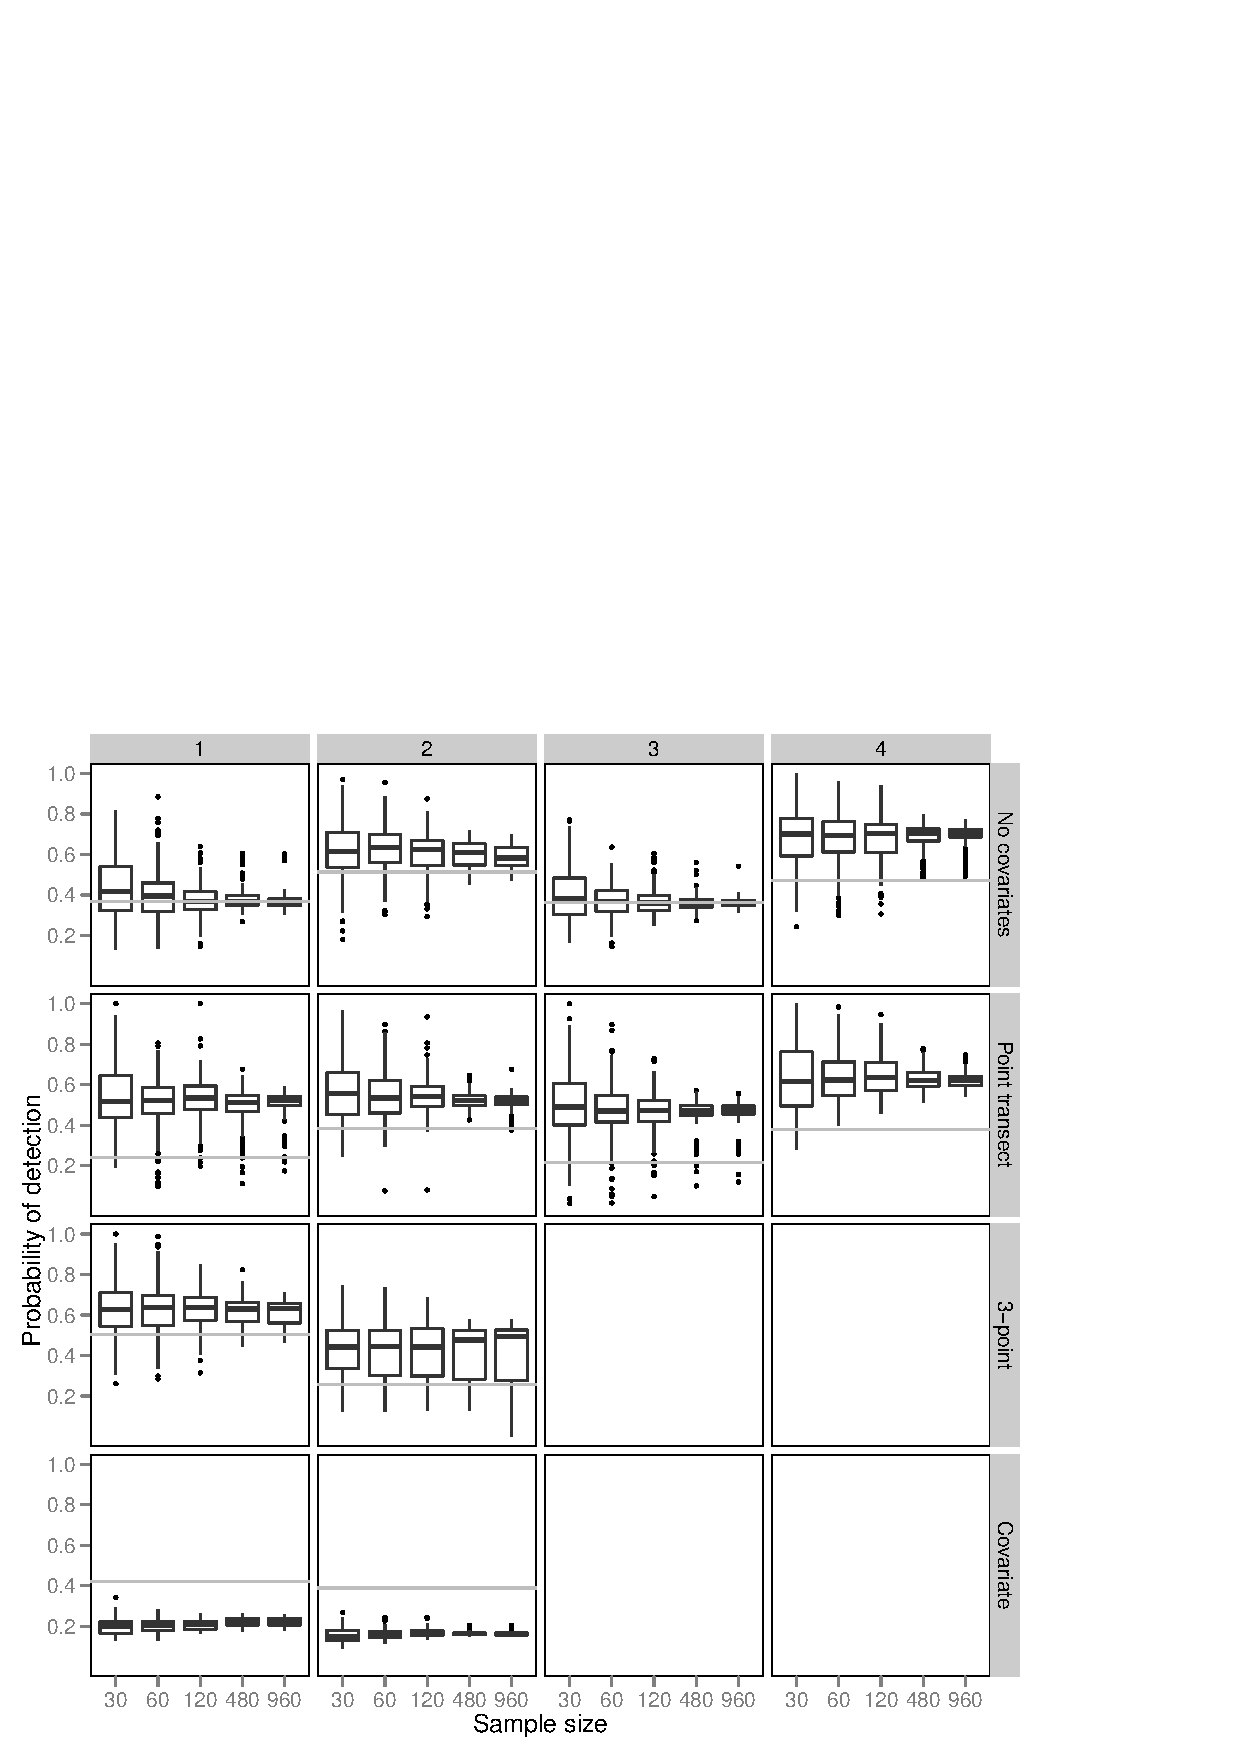
\includegraphics[width=\textwidth]{simulations/pa-plot-cds.pdf}
\caption{Simulation results: boxplots of the estimated average detection probabilities, $P_a$, for the best K+A model (by AIC score). Grey lines indicate the true value of the average detection probability.}
\label{sim-boxplots-cds}
\end{figure}

\begin{figure}[H]
\centering
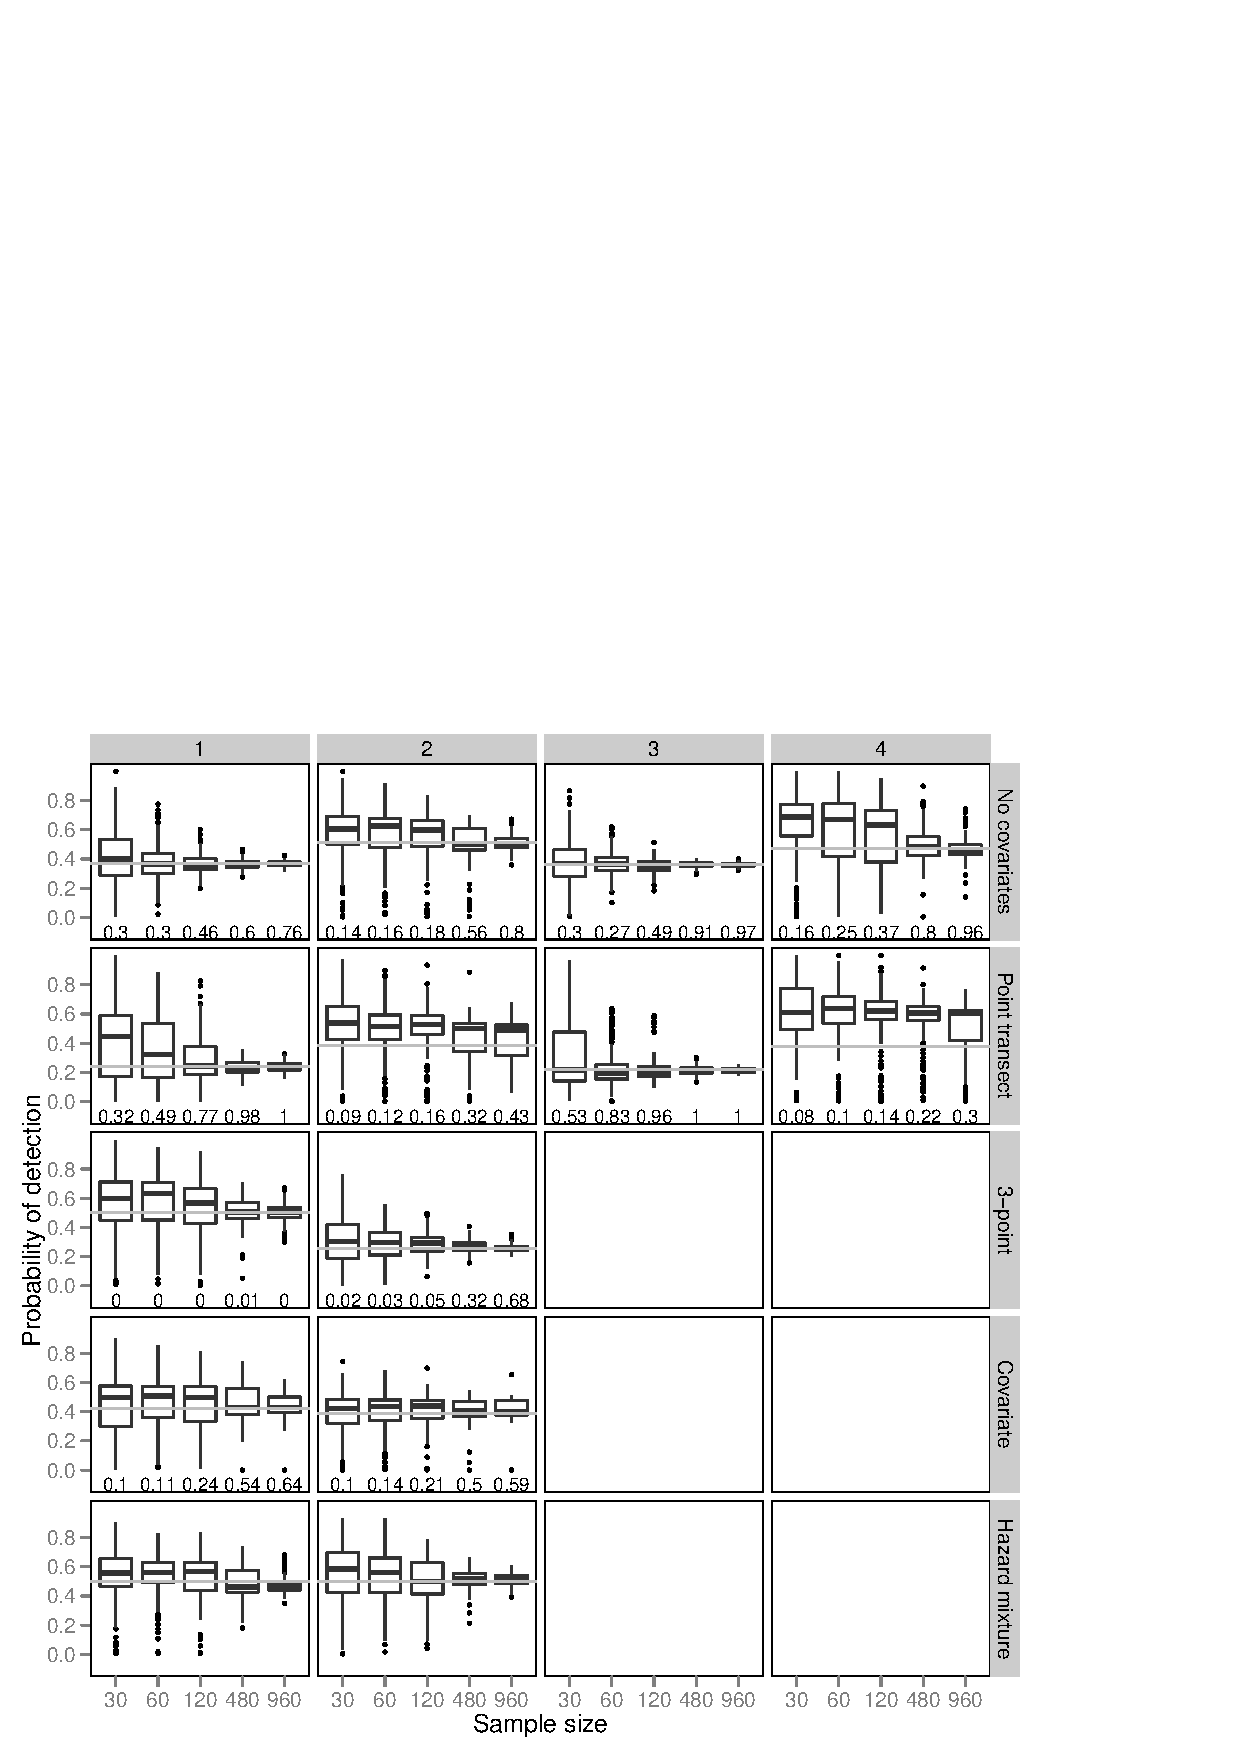
\includegraphics[width=\textwidth]{simulations/pa-plot-combined.pdf}
\caption{Simulation results: boxplots of the estimated average detection probabilities, $P_a$, for the best model (by AIC score) for both mixture and K+A models. In each case the best overall model was selected, reflecting the modelling approach undertaken in practice. Grey lines indicate the true value of the average detection probability. Numbers underneath each boxplot give the proportion of AIC best models that were of the same form as the model that the data was simulated from (e.g., in scenario D1, the proportion of AIC best models that were 2-point mixtures that included the covariate in the model). Numbers above each model give the proportion of times that the AIC best model was a 2- or 3-point mixture model.}
\label{sim-boxplots-combined}
\end{figure}

\begin{figure}[H]
\centering
\includegraphics[width=\textwidth]{simulations/bar-winners.pdf}
\caption{Simulation results: stacked bar charts showing the number of models selected by AIC that fall into the given model classes. Layout is as in Web Figure 3, above. ``hn'' is a half-normal detection function and ``hr'' is a hazard-rate detection function (no adjustments/1-point mixture). K+A indicates a key function plus adjustment term model where ``cos'' is cosine and ``poly'' are simple polynomial adjustments. MMDS is a mixture model with 2 or 3 components (``2-pt'' or ``3-pt'', respectively). ``(cov)'' indicates that covariates were included in the model (no adjustments were allowed when covariates were used).}
\label{sim-barplot}
\end{figure}


\newpage
\section*{Web Appendix F - Case studies}

Before analysing the wood ant and amakihi data the variables nest size (for ants) and minutes after sunrise (for amakihi) were standardised by dividing the variable by its standard error. 


\begin{figure}[H]
\centering
\includegraphics[width=0.3333\textwidth, trim=0 0 5.73228347in 0, clip=true]{analyses/ants-nesthab-1.pdf}\includegraphics[width=0.6666\textwidth, trim=2.86614173in 0 0 0, clip=true]{analyses/ants-nesthab-2.pdf}
\caption{Plot of the detection functions for the AIC best model for the ants data set (2-point mixture with nest size and habitat as covariates). The first panel shows the average detection function (dashed lines are the two mixture components of the detection function, averaged over covariate values). The second and third panels show the quartiles of nest size and the levels of habitat type respectively.}
\label{ants-nesthab}
\end{figure}

\begin{figure}[H]
\centering
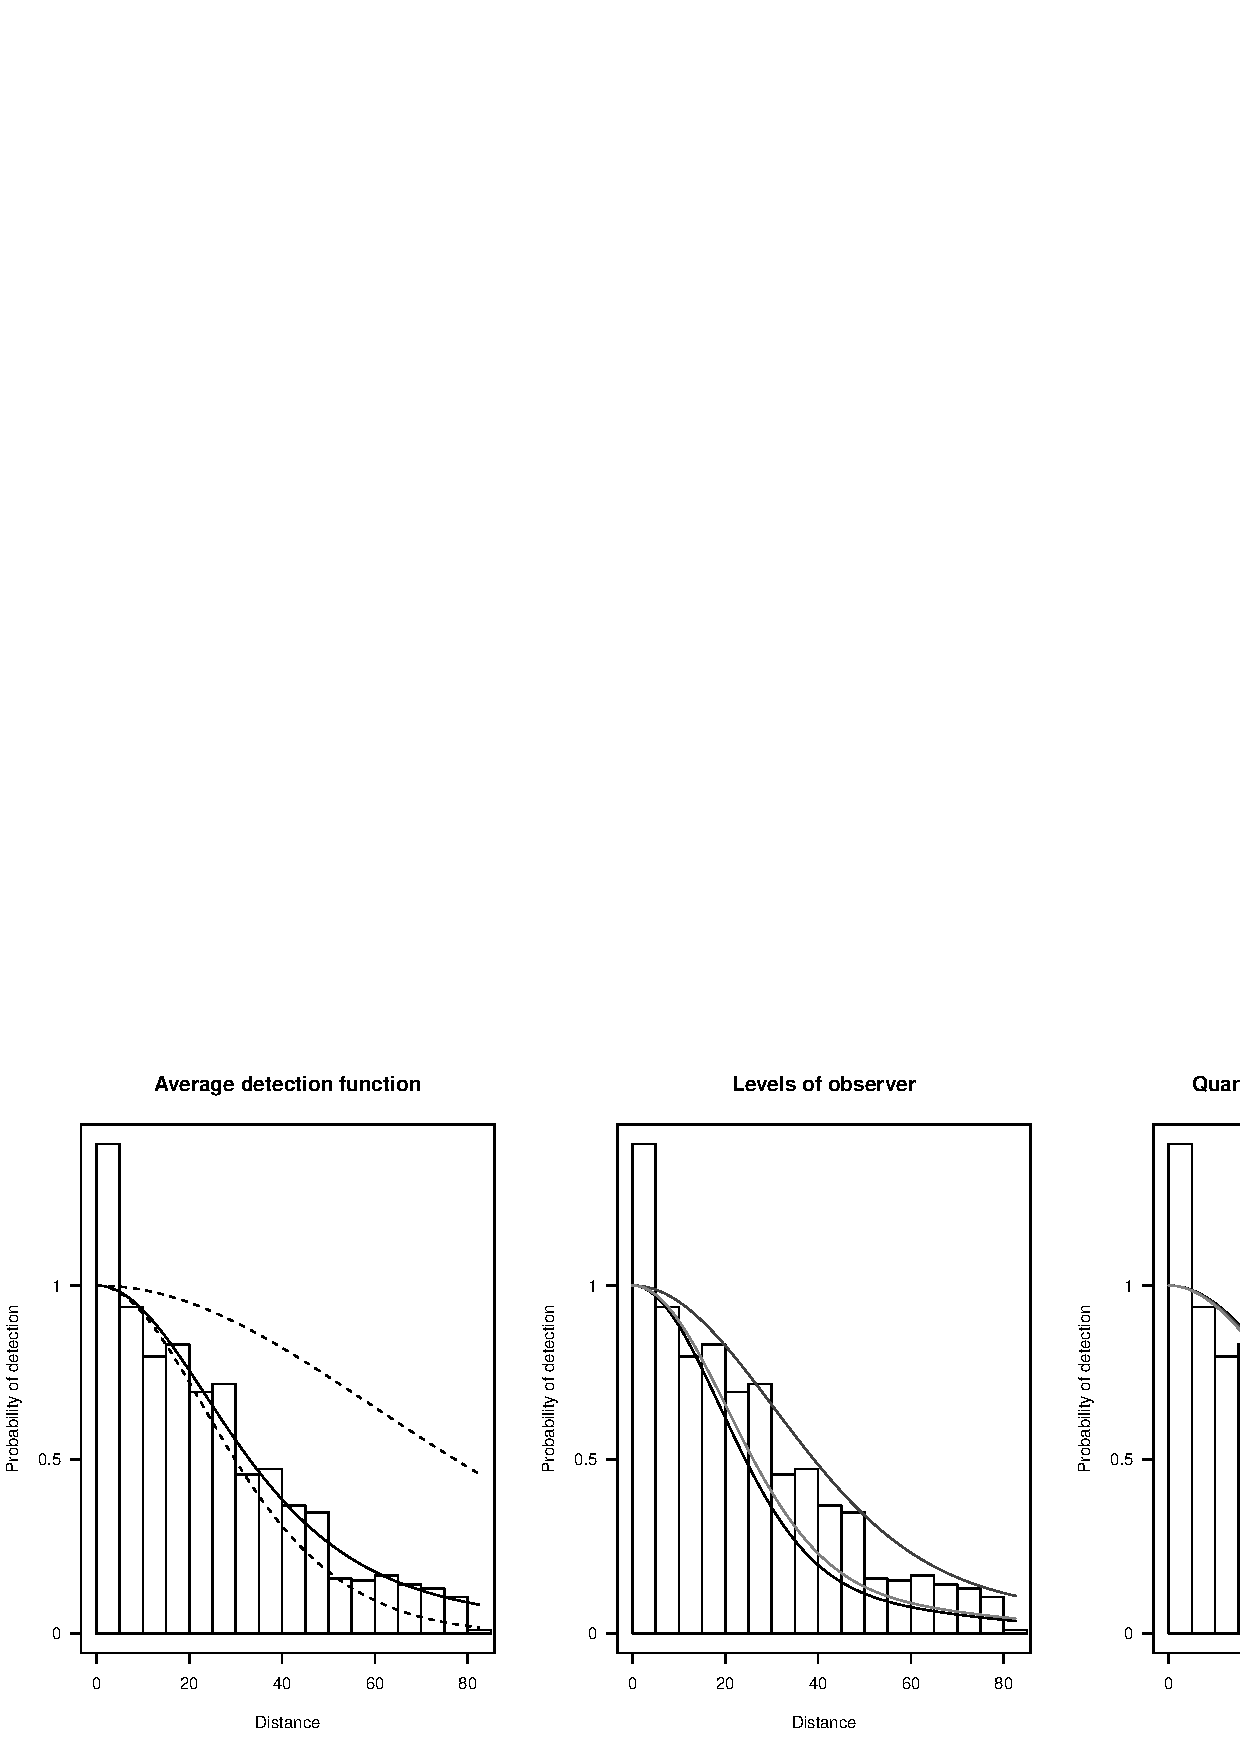
\includegraphics[width=0.3333\textwidth, trim=0 0 7.133334in 0, clip=true]{analyses/amakihi-om.pdf}\includegraphics[width=0.6666\textwidth, trim=3.566667in 0 0 0, clip=true]{analyses/amakihi-om-hh.pdf}\\
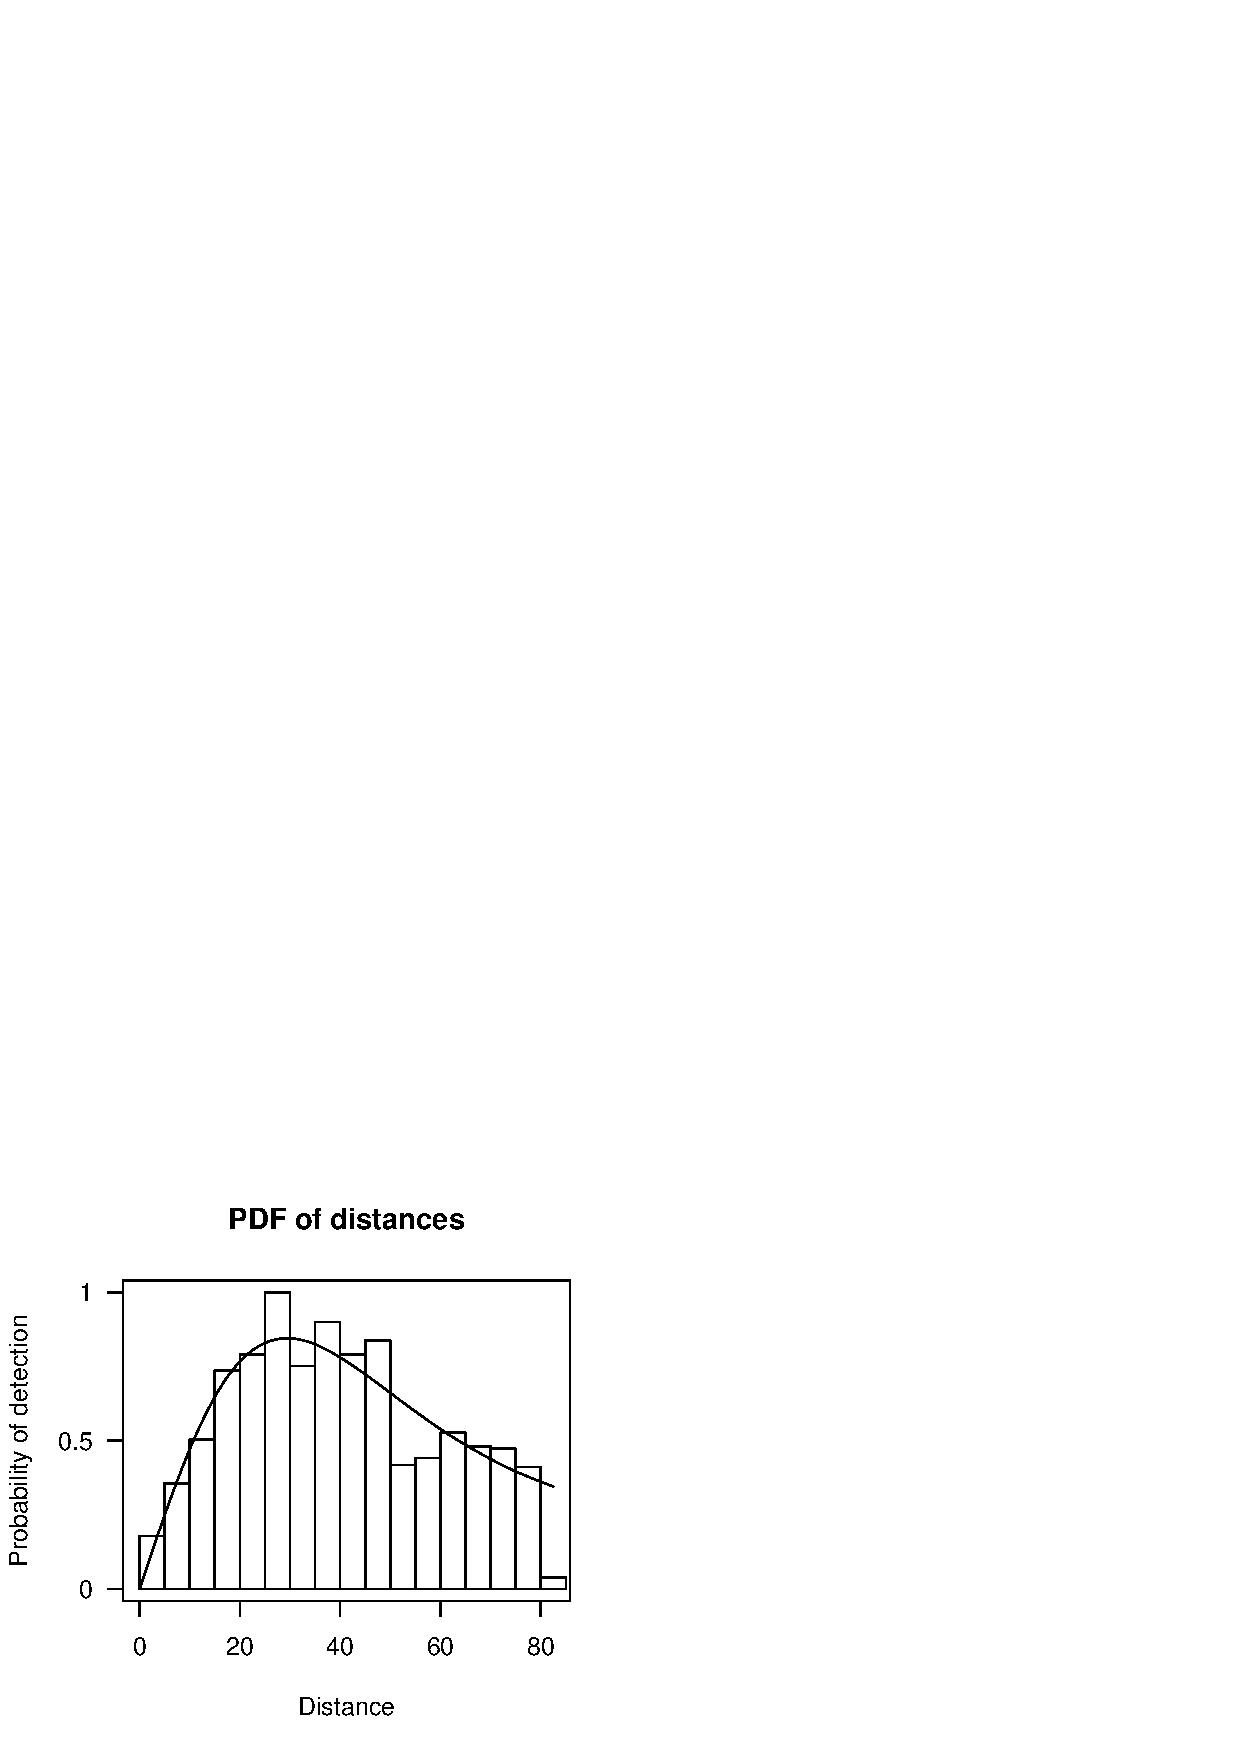
\includegraphics[width=0.4\textwidth]{analyses/amakihi-om-pdf.pdf}
\caption{Plots of the (AIC) best mixture model for the Amakihi data: a 2-point mixture with observer and minutes after sunrise as covariates. Top row: detection function averaged over covariates (dashed lines are each mixture component averaged over covariates), marginal detection function showing the levels of observer (averaged over the values of minutes after sunrise) and marginal detection function for minutes after sunrise ranging between 0 and 300 minutes (averaged over the levels of observer), as in Marques et al (2007). Bottom row: pdf of distances averaged over the covariate values.}
\label{amakihi}
\end{figure}


\bibliography{dsmixtures-appendix}

\end{document}